\section{Implementation}
\label{sec:eval}

The implementation of the three algorithms for empirical results has been done using the C++ programming language along with the Message Passing Interface standard (MPI). The experiments were carried out using the infrastructure provided by SHARCNET. The 64 bit high performance Opteron and Xeon clusters, consisted of a maximum of 16 nodes, with upto 4 cores on each node. The clusters run the Linux Operating system and are interconnected with each other through a private, dedicated connection running at 10 Gigabits per second. The complete implementation has been written in approximately $2$K lines of code. The source code for the same can be found at https://github.com/shreya-68/Consensus/tree/master/MPI. As a basic framework a synchronous peer-to-peer network was setup. On top of this network, the algorithms were implemented for testing purposes.  

\subsection{Input}
The input into the system is size of the network, i.e., total number of processes, along with the input value for each of the processes for achieving consensus. The ratio of number of byzantine processes to the number of good processes is provided as well along with a specified byzantine behavior. This behavior allows the byzantine processes to decide which values to send at every round of the protocol. 

\subsection{Output}
The output is the number of rounds carried out, CPU time utilization, runtime, number of messages/bits sent per node, and the final decision value of each process. 

\subsection{Testing parameters}
For testing the three algorithms, the number of processes $(n)$ lies in the range $4$ to $64$ on a cluster of $1$ to $16$ machines. The number of faults $(f)$ lies in the range $[0, n/3)$ for algorithms \textit{Pull-Push} and \textit{EIG}, and in the range $[0, n/4)$ for algorithm Quorum. These ranges have been considered since the algorithms have been shown to be correct only in these respective ranges.

\subsection{Authentication of processes}
It was assumed that the channels are authenticated and each receiving entity knows the identity of the sender. The communication primitives provided by the MPI library implicitly provide this functionality and hence, a byzantine process cannot spoof their identity or hide it.

\subsection{Connection}
Each process in the peer-to-peer network had full knowledge about the network connection of other processes, i.e., the IP address and port number of the hosts it was connected to. Using the MPI library this is done by giving a unique ID to each node from $[0, n)$. The MPI point-to-point operations were used for sending and receiving messages between any two, and only two processes. This behaves like a TCP connection and was used for reliable transfer of messages between hosts. It also guarantees order between messages but does not guarantee fairness. The implementation does not make use of any shared resources.

\subsection{Parallelization}
To allow programs to execute parts of the protocol that are independent of each other in parallel, MPI thread level support has been used. To further speedup the runtime, non-blocking calls have been used in some places where, for example, the execution of next few instructions does not depend on the completion of a send call. The MPI implementation creates a system buffer to typically hold data in transit. This is useful when a process wants to receive some messages sent to it by multiple other processes at a later time. This helped improve performance to an extent since it allows for send-receive operation to be asynchronous. Nevertheless, it is a finite resource and should be used carefully otherwise it can lead to loss of messages. 

\subsection{Byzantine behaviors}
The byzantine behaviors that a node can display are the following:
\begin{itemize}
    \item Crash failure: Processes may fail by stopping. Any good process that fails to send messages or aborts its execution is considered byzantine.
    \item Processes send conflicting data to different processes in the same round. Any data that is not the same or is null is said to be conflicting.
    \item Processes send arbitrary content or more messages than necessary. Byzantine processes may try to do so to choke the communication and flood the network or overload the requests that need to be answered.
    \item Denial of service: Byzantine processes may deny responding to requests from good processes or may not forward messages as required. 
\end{itemize}

\subsection{Synchronization}
To implement a synchronous model of communication, we make use of communicators, that is essentially a group of processes. A synchronisation operation, \texttt{MPI\_Barrier} is a routine provided by the MPI library. It allows one to specify a group to wait on. A process blocks on this call until all processes in the specified group reach this call. To keep all the processes in the network synchronized after each phase, this routine is used whose group is set to the active processes in the network.



\subsection{Fault Tolerance against crash failures}
One assumption that is made throughout is that once a process suffers a crash failure, it cannot recover from it. An advantage of using TCP connections was that it allowed failure discovery in the case of a crash failure. If a process failed before the start of a phase, it would not communicate with any process in the next phase and neither would any other process be able to establish a connection with it. This led to failure discovery. If a process crashed within a phase, the wait groups helped in failure discovery. A timeout mechanism was used to implement this. Each phase had to be completed within a certain amount of time and if all the processes did not reach the synchronisation operation within that allotted time, it indicated that a process was down and the other processes proceeded with the next phase. This mechanism worked since we were not dealing with more than $64$ processes and by running the system multiple times we could determine what the timeout value should be such that, with high probability, alive processes are allowed to finish the phase. An alternative to this method was sending an acknowledge back but, we refrained from using this method since that meant dealing with twice the number of messages which added unnecessary overhead for our testing purposes. 

\subsection{Message format}
Each message sent over the network was an array of bytes of the following form:
\begin{equation*}
    \mathtt{LENGTH}, \mathtt{PHASE}, \mathtt{MESSAGE}
\end{equation*}
The $\mathtt{LENGTH}$ parameter indicated how many bytes of the message to parse. The $\mathtt{PHASE}$ parameter indicated which phase the message was sent during and also what its purpose in that phase is. As in the algorithm \textit{Pull-Push}, the pull phase sends messages of type `ANSWER', `ROUTE', `FORWARD' and so on. The format of the $\mathtt{MESSAGE}$ varied for each of the algorithms.


\section{Results}
\label{sec:results}

\subsection{Bit Complexity}
For the \textit{EIG} algorithm, from Fig. \ref{fig:eig}, we can see that as the network size increases the bit complexity only increases as a cubic function in accordance with the theoretical Big `O' complexity of $O(n^3 logn)$, where $n$ is the size of the network. This is a major improvement from classic deterministic algorithms that have very high polynomial growth. One can note from Fig. \ref{fig:eignolog} that the fault ratio affects the bit complexity by a factor of $n$. This is because the higher the ratio, faulty nodes try to dominate the number of bits a good process receives by claiming all processes are byzantine in every round. They send $n^2$ bits of information in every round to every other process. Whereas, good processes only send $n*k$ bits of information. As the number of processes start to increase the trends for each of the fault ratios becomes similar. However, for small networks, the bit complexity is quite diverse for different fault ratios. This shows that for systems with high variable size of the network, any fault ratio will affect the bandwidth comsumption in a similar manner but, for small networks with varying fault ratios the bandwidth consumption could be affected greatly.   
\begin{figure}[h]
 \centering
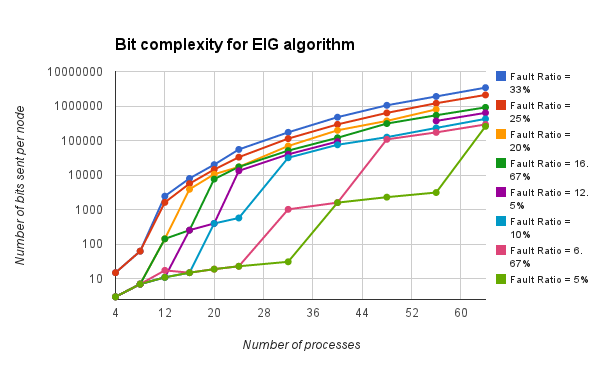
\includegraphics[scale=0.4]{eig}
\caption{Consensus results for EIG algorithm (Log Scale)}
 \label{fig:eig}
\end{figure}

\begin{figure}[h]
 \centering
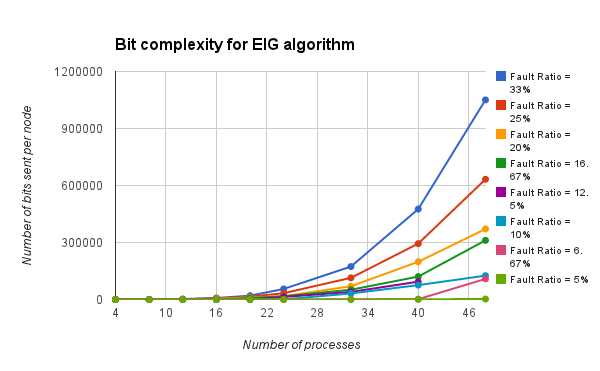
\includegraphics[scale=0.4]{eignolog}
\caption{Consensus results for EIG algorithm}
 \label{fig:eignolog}
\end{figure}
For the \textit{Pull-Push} algorithm, as the network size increases the bit complexity displays a polylogarithmic growth. The growth trend is similar for all fault ratios for small and larger networks. The increase in number of faults has an effect on the number of bits sent per node but only by a constant factor. This is can be attributed to the fact that in the protocol, even if byzantine nodes try to send conflicting values and arbitrary number of them to samplers for the purpose of flooding, the samplers do not receive enough of them to forward these messsages further in the protocol. This can be see from Fig. \ref{fig:pull_push}. Also note that, for networks with $logn$ remaining the same, the bits sent per node is the same and it only changes at network sizes that are powers of $2$. This is because good processes only communicate with samplers of size $logn$. Hence, for larger networks, increasing the size of the network by less than $100\%$ will not affect the bandwidth consumption.
\begin{figure}[h]
 \centering
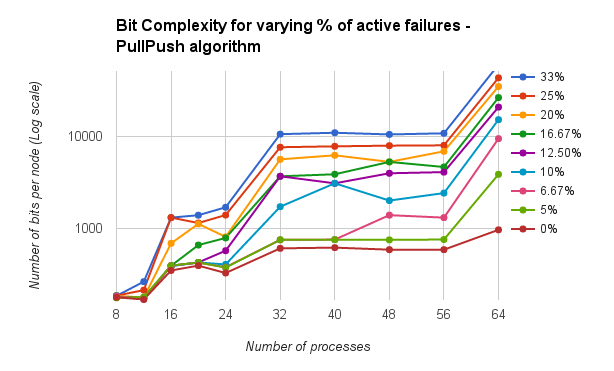
\includegraphics[scale=0.4]{pull_push}
\caption{Consensus results for Pull-Push algorithm (Log scale)}
 \label{fig:pull_push}
\end{figure}

The \textit{Quorum} algorithm shows very high bits per node communication even for small networks. It increases rapidly as the network size increases. The reason for this is that Gradecast requires all-to-all communication between processes and the protocol requires processes to run a deterministic BA protocol for every subset of a committee in Stage $2$ of the protocol. The fault ratios do not have much of an effect on the communication costs. Byzantine nodes are unable to increase bits on the network by participating in more subprotocols than the algorithm requires since, membership in a subprotocol is dictated by their ID which is fixed. Hence, more number of nodes are unable to influence the communication cost greatly which is high anyway.  
\begin{figure}[h]
 \centering
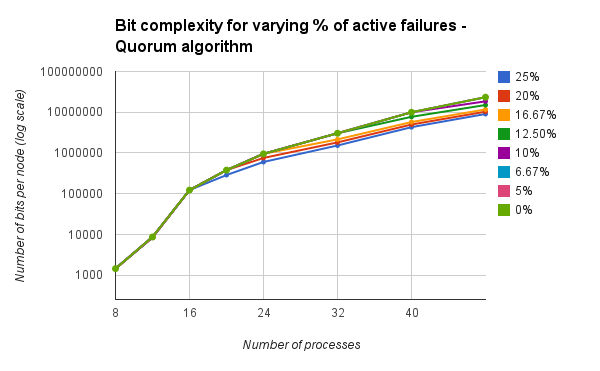
\includegraphics[scale=0.4]{quorum}
\caption{Consensus results for Quorum algorithm}
 \label{fig:quorum}
\end{figure}

Each of our algorithms for every configuration was run $5$ times and we obtained confidence intervals for each of them. The confidence interval for algorithm \textit{Pull-Push} was $\pm 1\%$, for algorithm EIG - $\pm 0.1\%$, and $\pm 0.5\%$ for algorithm Quorum.

\subsection{Comparison}
We now compare the relative performance of each algorithm. For large networks ($n > 64$), we vary the ratio of faults to the number of processes ($f/n$), which lies in the range $[0, 1/3)$ for algorithms \textit{EIG} and \textit{Pull-Push} and in the range $[0, 1/4)$ for algorithm \textit{Quorum}.
As can be seen from Fig. \ref{fig:comp}, the algorithm Pull-Push performs much better, than the other algorithms even for maximum allowed faulty processes.

We modify the \textit{EIG} protocol a little and require that instead of sending the complete byzantine list every time, from round $4$ onwards only the changes to this list be sent in every round. This does not change the correctness of the algorithm since all the good nodes send the same changes to every other process in a round and in the next round the confirmation mechanism would confirm these updated lists. The rest of the algorithm works in the same way. Even though this does not change the communication complexity in the worst case, it overall reduces the communication bits as good nodes would send a bit for every suspected byzantine node only in any one of the rounds instead of every round. This modified version of the algorithm performs much better. For small ratios since the number or rounds is small, the number of bits sent per node remains the same but it does not vary a great amount as the ratio increases.
\begin{figure}[h]
 \centering
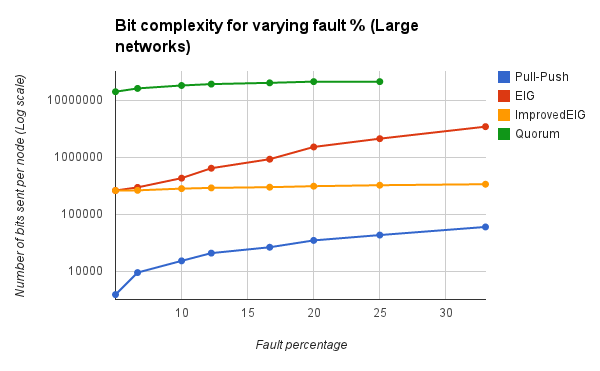
\includegraphics[scale=0.4]{LargeNetBit}
\caption{Comparison for large networks}
 \label{fig:comp}
\end{figure}

\begin{figure}[h]
 \centering
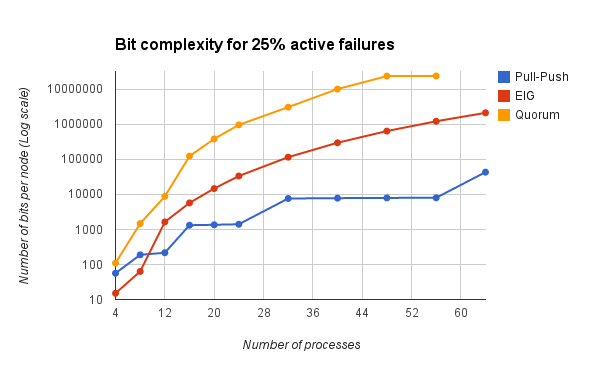
\includegraphics[scale=0.4]{Fault25}
\caption{ Comparison for variable number of faults in each algorithm}
 \label{fig:fault25}
\end{figure}

\begin{figure}[h]
 \centering
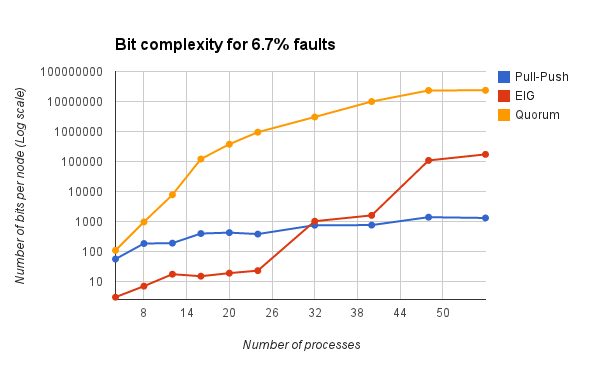
\includegraphics[scale=0.4]{Fault667}
\caption{ Comparison for variable number of faults in each algorithm}
 \label{fig:fault667}
\end{figure}

\begin{figure}[h]
 \centering
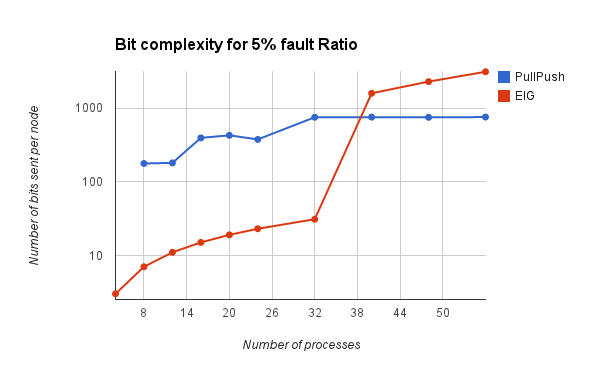
\includegraphics[scale=0.4]{Fault5}
\caption{ Comparison for variable number of faults in each algorithm}
 \label{fig:fault5}
\end{figure}

For small networks ($n < 40$), if the fault ratio is small and in the range $[0, 1/15)$, Figs. \ref{fig:fault667} and \ref{fig:fault5} show that algorithm \textit{EIG} performs much better than any of the other algorithms. This is simply because only the first three rounds of this algorithm will be executed and since the ratio is small, a simple broadcast is sufficient to gather all the information. Pull-Push and Quorum, more complex algorithms, perform worse in such scenarios. Fig. \ref{fig:fault25}, shows that for higher fault ratios and any network size algorithm Pull-Push performs better.

Depending on the system requirements such as how fast we want the information to reach the destination, bandwidth and so on, there were two mechanisms we used to send the messages. In an algorithm like Pull-Push, where multiple message packets maybe sent to the same node by a process in the same round, one could marshall all the packets into one packet and then send it. This obviously comes at the cost of parallelization where one has to first wait to receive all the messages from the previous round, perform operations and then send out messages all at once. While the number of messages sent per node changed on using the latter method, the number of bits sent remained the same.

%The difference in the number of messages sent for the two mechanisms can be seen in Fig. \ref{fig:opt}.
%\begin{figure}[h]
% \centering
%\includegraphics[scale=0.55]{optimized}
%\caption{ EIG algorithm when messages are grouped before sending}
% \label{fig:opt}
%\end{figure}

\subsection{Round Complexity}
Round complexity is the number of phases that have to be executed sequentially by a processes and one cannot parallelize these phases. For example, in algorithm EIG, a round consists of broadcast of messages at the same level $i$ in the EIG trees by each process. For algorithm Quorum, a round consists of broadcast of messages during a particular subprotocol. There are two outlooks to analyzing the round complexity of this algorithm. The first is that each of the subprotocols $S_i^j$ could be executed in parallel since none of these subprotocols are dependent on each other. Hence, all of them together make one round. But, parallel execution of these subprotocols is not possible due to resource constraints then each of them is an independent round. For algorithm Pull-Push, the push phase makes one round and sending, routing and answering in the pull phase form imdependent rounds.

A comparison of the round complexities can be seen in Figs. \ref{fig:round6} and \ref{fig:round16} for fault percentage $~6.5\%$ and $~16.5\%$, respectively. In both the figures parallel execution of subprotocols for algorithm Quorum is assumed. 

\begin{figure}[h]
 \centering
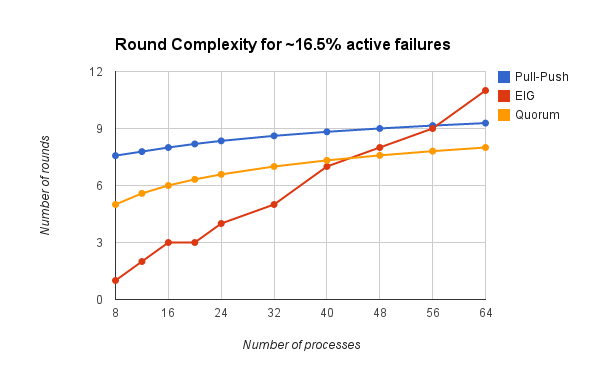
\includegraphics[scale=0.4]{Round16}
\caption{Time Complexity comparison}
 \label{fig:round16}
\end{figure}

\begin{figure}[h]
 \centering
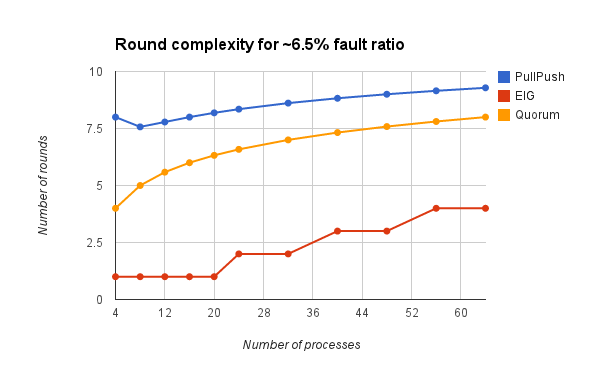
\includegraphics[scale=0.4]{Round6}
\caption{Time Complexity comparison}
 \label{fig:round6}
\end{figure}

\subsection{Time Complexity}

For relative performance comparison of time utilisation, we compare the CPU times and runtimes of the execution of each algorithm.  From figures \ref{fig:cpu} and \ref{fig:elapsed} we see that CPU time utilisation and running time of EIG increases rapidly and it is a lot slower compared to the other two algorithms. If we look at the runtimes, we can see that algorithm Quorum remains the fastest throughout. This is because Quorum is highly parallel. The trade-off here is that the CPU time utilisation of \textit{Quorum} is a lot more than that of \textit{Pull-Push}. This trend is maintained for all fault ratios.

\begin{figure}[h]
 \centering
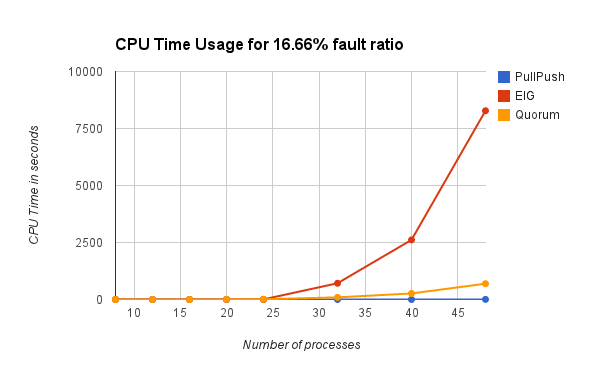
\includegraphics[scale=0.4]{cpu16}
\caption{Time Complexity comparison}
 \label{fig:cpu}
\end{figure}

\begin{figure}[h]
 \centering
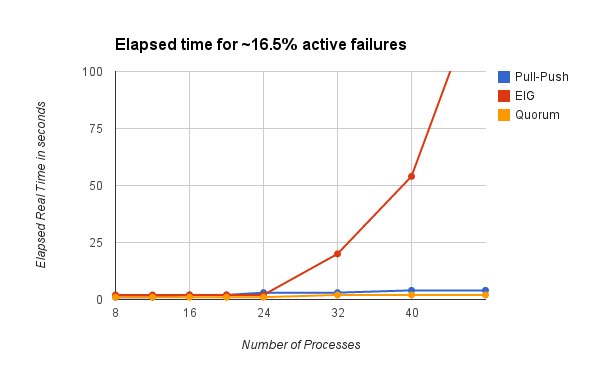
\includegraphics[scale=0.4]{elapsed16}
\caption{Time Complexity comparison}
 \label{fig:elapsed}
\end{figure}

%Fig. \ref{fig:time} the first mechanism for calculating time complexity of algorithm Quorum is used, where it is considered that all the subprotocols together form one round. This figure shows the algorithm Quorum gives better performance than algorithms EIG and Pull-Push as the number of processes in the network increases. Also, algorithm Pull-Push diverges in complexity due to increasing number of candidate strings that could be injected by the adversarial processes.

%Fig. \ref{fig:time_nopar}, shows a comparison of time complexities if each subprotocol in algorithm Quorum is treated as an individual round. In contrast to Fig. \ref{fig:time}, this figure clearly shows that the time complexity of algorithm Quorum increases rapidly, whereas for algorithms EIG and Pull-Push there is no drastic increase. Hence, if resources are limited and parallel processing of each subprotocol is not possible, algorithm Quorum does not give good performance.
%
%\begin{figure}[h]
% \centering
%\includegraphics[scale=0.55]{time_nopar}
%\caption{Time Complexity comparison no parallel execution}
% \label{fig:time_nopar}
%\end{figure}


\subsection{Discussion}

In real-world applications, achieving distributed consensus has become increasingly important. In most cases, consensus is only a small but frequently used sub-component of a larger protocol such as in distributed databases. Thus, improving the communication and time complexity of this algorithm is essential to the overall performance of such systems. One needs to consider implementation issues that come along with any of these algorithms and not only their theoretical results. During implementation, one can improve certain tasks such as sending a larger message instead of many smaller messages or executing parallelizable tasks at the same time on multi-core machines.  

As can be seen from the figures above, according to the requirements and resources available, each algorithm gives different performance. Once we have an algorithm to implement, the first thing to consider before implementation is what resources we have and how can we design the system such that we get optimal results for the available resources. Implementing the testbed framework on a cluster allowed us to mimic real-time scenarios. We considered different byzantine behaviors and during execution if any good process crashed due to unknown reasons we included it as a byzantine process. To report on the maximum number of bits sent per node, we considered byzantine processes that were trying to flood the network. On executing hte algorithms in the case of a denial of service attack, an increasing ratio of faulty processes reduced the communication overhead instead of increasing it. Crashing failures also reported similar results. If the faulty processes only sent out arbitrary messages, the algorithms executed correctly without hampering the communication cost too much if the ratio of byzantine processes was increased.

Another optimization that would have save the running time of the system would be to use UDP connections instead of TCP since they take up less resources and provide lesser overhead. Even though UDP connections do not guarantee message delivery, for a small system it could be considered highly reliable still. The rationale behind using TCP connections for this testbed framework was to model and understand implementation issues for more realistic distributed applications, which could have peers separated by geographical distance. In such cases, TCP connections provide greater reliability. 

An analysis of the three algorithms and their performance for a wide range of number of processes and faults shows that communication of each process with fewer number of processes yields good results instead of all-to-all communication. This inhibits byzantine processes from influencing values of too many good processes. It is also important that requests from byzantine processes be throttled at an early stage. The good performance of the deterministic algorithm for small fault ratios shows that it is important to consider this factor when designing an algorithm.  Communication between multiple sets of quorums allows parallel tasks to be executed and gives good time complexity results. The combined use of these techniques might help us design improved algorithms in the future to solve the problem of distributed consensus. 




